\documentclass[11pt]{beamer}
\usetheme{CambridgeUS}
\usepackage[utf8]{inputenc}
\usepackage{amsmath}
\usepackage{amsfonts}
\usepackage{amssymb}
\usepackage{graphicx}
\author{Mr.BOURZIK abdelati}
\title{Les réseaux Mobile Ad Hoc MANET}
%\setbeamercovered{transparent} 
%\setbeamertemplate{navigation symbols}{} 
\logo{USMS FP BM} 
\institute{\emph{UniversitySoltan moulay Sliman\\
Faculté Polydiscplinaire Beni Mellal}}
\date{1 december 2020}
%\subject{} 
\begin{document}
\begin{frame}
\titlepage
\end{frame}
\section*{sommaire}
\begin{frame}\frametitle{Plan de l'exposé}
\tableofcontents[hideallsubsections,pausesections]
%\begin{onlyenv}<1->{}\tableofcontents[hideallsubsections,pausesections]\end{onlyenv}
%\temporal<1->{}{\tableofcontents[hideallsubsections,pausesections]}{} 
%\pause[2]
%\onslide<2->{\tableofcontents[hideallsubsections,pausesections]}
\end{frame}
\section{A qoi sert MANET}
\begin{frame}{Mobile Ad hoc Network}
Mobile ad hoc networks ou MANET, est le nom d'un groupe de travail de l'IETF, créé en 1998-1999, chargé de standardiser des protocoles de routage basés sur la technologie IP pour les réseaux ad hoc sans fil. MANET fait aussi référence aux réseaux sans infrastructure dans lesquels toutes les stations peuvent être mobiles.
\\
le nom propre MANET est parfois utilisé comme nom commun pour désigner un réseau ad hoc, spécialement dans les pays anglophones.\\
MANET stands for Mobile adhoc Network also called as wireless adhoc network or adhoc wireless network that usually has a routable networking environment on top of a Link Layer ad hoc network.. They consist of set of mobile nodes connected wirelessly in a self configured, self healing network without having a fixed infrastructure. MANET nodes are free to move randomly as the network topology changes frequently. Each node behaves as a router as they forward traffic to other specified node in the network.
\end{frame}
\section{Characteristics of MANET }
\begin{frame}{les caractéristiques}
\begin{itemize}
\item \textbf{Dynamic Topologies:} Network topology which is typically multihops, may change randomly and rapidly with time, it can form unidirectional or bi-directional links.
\item \textbf{Bandwidth constrained, variable capacity links:} Wireless links usually have lower reliability, efficiency, stability, and capacity as compared to wired network. The throughput of wireless communication is even less than a radio’s maximum transmission rate after dealing with the constraints like multiple access, noise, interference conditions, etc.
\item \textbf{Autonomous Behavior:} Each node can act as a host and router, which shows its autonomous behavior.
\end{itemize}
\end{frame}
\begin{frame}{les caractéristiques}
\begin{itemize}
\item \textbf{Energy Constrained Operation:} As some or all the nodes rely on batteries or other exhaustible means for their energy. Mobile nodes are characterized with less memory, power, and lightweight features.
\item \textbf{Limited Security:} Wireless network are more prone to security threats. A centralized firewall is absent due to its distributed nature of the operation for security, routing, and host configuration.
\item \textbf{Less Human Intervention: }They require minimum human intervention to configure the network, therefore they are dynamically autonomous in nature.
\end{itemize}
\end{frame}
\section{Domaines d'application du MANET}
\begin{frame}{Applications Manet}
les applications de réseaux mobiles sans files ad hoc sont nombreux, parmi ses applications on trouve :\\
\begin{itemize}
\item \textbf{Militaires}
\item \textbf{Urgences}
\item \textbf{VANET}
\item \textbf{Applications collaborative}
\item \textbf{Jeux videos}
\item \textbf{PAN}
\end{itemize}
\end{frame}
\begin{frame}
\begin{exampleblock}{Militaires}
le développement de PRN ou Packet Radio Networks, qu'est conçu pour l’armée américaine, permet de déployer une infrastructure de communication entre chaque bataillon, par l’intermédiaire de plusieurs véhicules communiquant ensemble.\\
lors d'iterventions en milieu hostile, les réseaux Manet sont bien adaptés à ce type d'envirinnement où les déplacements restent rapides, exemple:\\
\centering
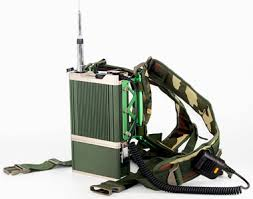
\includegraphics[scale=0.45]{img2.jpg}
\begin{figure}
\caption{telecommunication device}
\end{figure} 
\end{exampleblock}
\end{frame}
\begin{frame}
\begin{exampleblock}{Urgences}
Les réseaux mobiles sans fil Ad-Hoc pourraient être utilisés dans les cas d’urgence et les opérations de recherche et secours lors d’un désastre (feux, inondation, séisme). Ces
opérations de secours peuvent parfois avoir lieu là où les infrastructures de télécommunication sont inexistantes, endommagées ou lors d’un besoin de déploiement rapide.
Cette infrastructure de télécommunication contient les services \textbf{GETS} (Government
Emergency Telecommunications Service),\textbf{TSP} (Telecommunications Service
Priority) et \textbf{WPS} (Wireless Priority Service) de \textbf{NCS} (National Communications System).
\end{exampleblock}
\end{frame}
\begin{frame}
\begin{exampleblock}{les réseaux VANET}
Dans le domaine routier,Manets peut nous aider pour la distribution d’information au niveau local (risque d’accidents ou d’encombrements), aide automatique à la conduite, téléphonie entre véhicules.\\
\centering
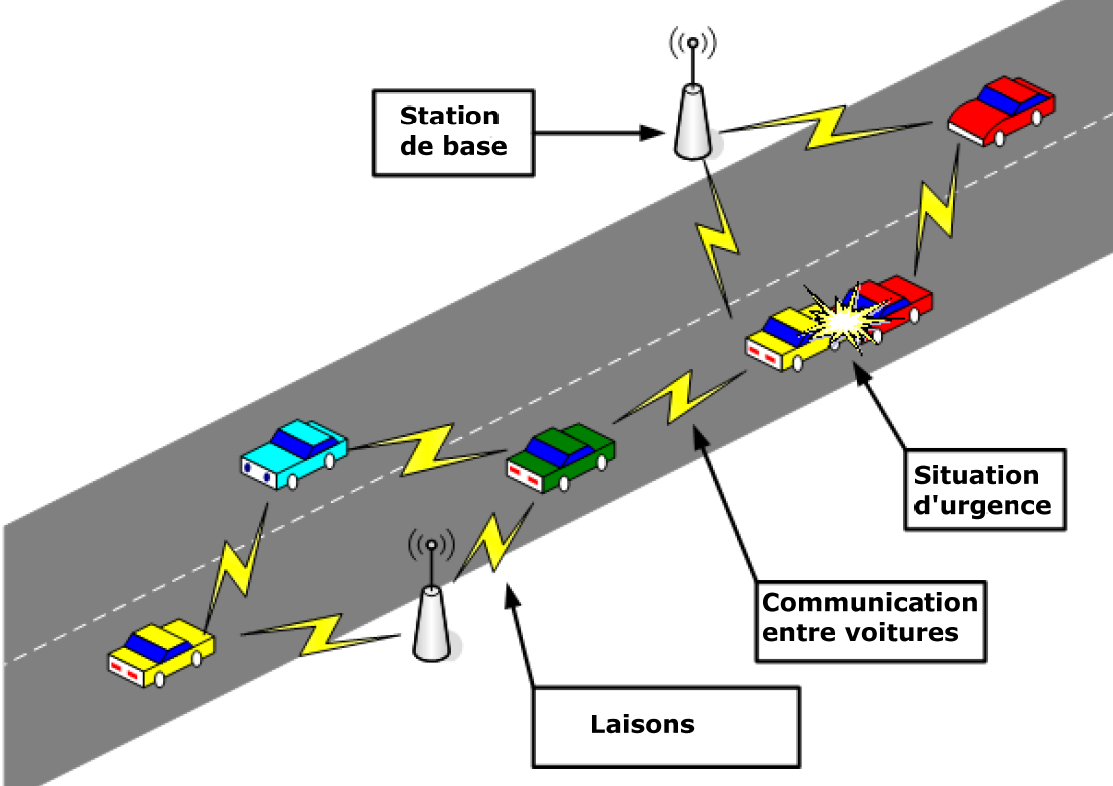
\includegraphics[scale=0.3]{Vanet.png}
\begin{figure}
\caption{surveillance du trafic routier }
\end{figure} 
\end{exampleblock}
\end{frame}
\begin{frame}
\begin{exampleblock}{Applications de collaborations}
Les réseaux ad hoc peuvent aussi être utilisés pour relier plusieurs ordinateurs entre-eux. et l'échanges d'informations entre les collaborateurs, ou faire des vidéos conférences entre bureaux voisins.
\end{exampleblock}
\begin{exampleblock}{Jeux vidéo}
C'est pour les utilisaeurs voulant jouer en réseau,Sony a offert en 2008 le premier modèle de console de jeu portable \textbf{PSP} permettant le jeu en réseau grâce à la technologie Ad-Hoc.\\
\centering
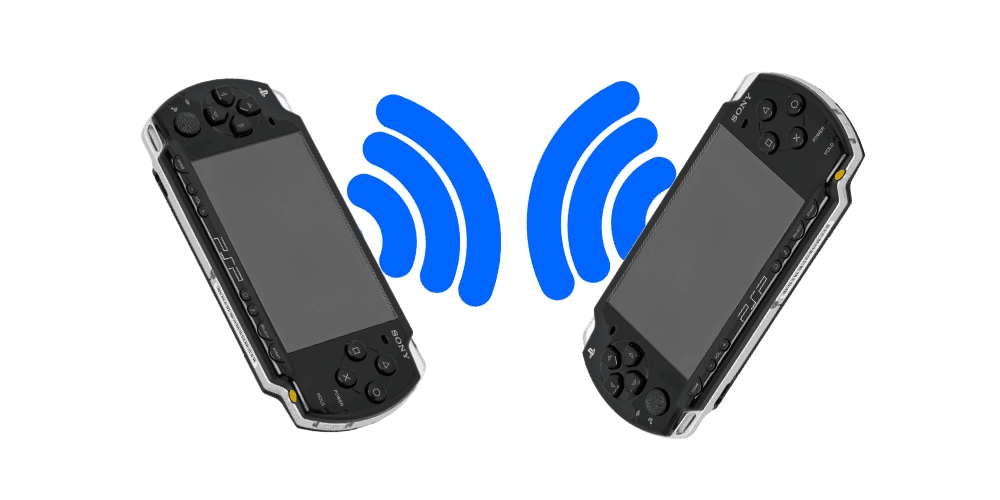
\includegraphics[scale=0.13]{img1.PNG}
\begin{figure}
\caption{PSP-Multiplayer games}
\end{figure}
\end{exampleblock}
\end{frame}
\begin{frame}
\begin{exampleblock}{les réseaux PAN}
Les réseaux mobiles sans fil Ad-Hoc pourraient être utilisés pour simplifier l'intercommunication et le partage des applications entre plusieurs équipements mobiles
(ordinateur portable, téléphone cellulaire ou autres) dans une zone limitée qu’on appelle Personal Area Network (PAN).
\end{exampleblock}
\end{frame}
\section{Types of MANET }
\begin{frame}{les types de Manet}
\begin{enumerate}
\item \textbf{Vehicular Ad hoc Network (VANETs):}Enable effective communication with another vehicle or with the roadside equipments.Intelligent vehicular ad hoc networks(InVANETs) deals with another vehicle or with the roadside euipments.
\item \textbf{Smart Phone Ad hoc Network (SPANC):}To create peer-to-peer network without relying on cellular carrier networks, wireless access points or traditional network infrasture.Here peer can join or leave the network without destroying it.

\item \textbf{Internet based Mobile Ad hoc Network (iMANETs):}It supports internet protocols such as TCP/UDP and IP. To link mobile nodes and establish routes distributed and automatically.

\item \textbf{}
\end{enumerate}
\end{frame}
\begin{frame}{les types de Manet}
\begin{enumerate}
\item \textbf{Hub-Spoke MANET:}Multiple sub MANET’s may be connected in hub-spoke VPN to create a geographically destributed MANET. Normal Ad-hoc routing algorithm does not apply directly.
\item \textbf{Military or Tactical MANETs:}This is used by the military units. Emphasis on data rate, real time demand, fast re-routing during mobility, security, radio range, etc.
\item \textbf{Flying Ad hoc Network (FANETs):}This is composed of unmanned aerial vehicle (commonly known as drone). Provides links to remote areas and mobility.
\end{enumerate}
\end{frame}
\section{Pros and Cos }
\begin{frame}{avantages}
\begin{itemize}
\item[\textbf{::}]Separation from central network administration.
\item[\textbf{::}]Each nodes can play both the roles ie. of router and host showing autonomous nature.
\item[\textbf{::}]Self configuring and self healing nodes, does not require human intervention.
\end{itemize}
\end{frame}
\begin{frame}{inconvinion}
\begin{itemize}
\item[\textbf{::}]Resources are limited due to various constraints like noise, interference conditions, etc.
\item[\textbf{::}]Lack of authorization facilities.
\item[\textbf{::}]More prone to attacks due to limited physical security.
\end{itemize}
\end{frame}
\end{document}